% Supplementary material for capstone_rp.tex, in the same IEEEtran format as the
% main paper, with S-prefixed numbering throughout.
% Tables in tables.tex are generated by make_tables.py; do not edit them by hand.
% Result tables are from the single G-12 test campaign (results/g12/).
% Code excerpts are taken from the repository at commit d5336cd with input
% validation removed for brevity; the logic is otherwise unchanged.
\documentclass[conference]{IEEEtran}

\usepackage{amsmath,amssymb}
\usepackage{booktabs}
\usepackage{graphicx}
\usepackage[ruled]{algorithm2e}
\usepackage{listings}
\usepackage{xcolor}
\usepackage{placeins}
\usepackage{microtype}
\usepackage[hidelinks]{hyperref}
\graphicspath{{../figures/}{figures/}}

% S-prefixed numbering so nothing here can be confused with the main paper.
\renewcommand{\thesection}{S\arabic{section}}
\renewcommand{\thetable}{S\arabic{table}}
\renewcommand{\thefigure}{S\arabic{figure}}
\renewcommand{\thealgocf}{S\arabic{algocf}}
\AtBeginDocument{\renewcommand{\thelstlisting}{S\arabic{lstlisting}}}

% Algorithm boxes: "ALGORITHM S1: Title" between rules, italic comment lines.
\SetAlgorithmName{Algorithm}{algorithm}{List of Algorithms}
\SetAlgoCaptionSeparator{:}
\SetAlCapFnt{\footnotesize\scshape}
\SetAlCapNameFnt{\footnotesize}
\SetAlFnt{\footnotesize}
\SetAlgoLined
\DontPrintSemicolon
\SetKwInput{KwIn}{input}
\SetKwInput{KwOut}{output}
\SetKwProg{Fn}{function}{}{}
\SetKw{KwVar}{var}
\SetKw{KwTo}{to}
\SetKwComment{tcp}{}{}
\SetCommentSty{textit}
\SetKwFunction{KeyedNoise}{KeyedNoise}
\SetKwFunction{PeakProject}{PeakProject}

\definecolor{codegray}{gray}{0.45}
\lstset{
  language=Python,
  basicstyle=\ttfamily\scriptsize,
  keywordstyle=\bfseries,
  commentstyle=\color{codegray}\itshape,
  stringstyle=\color{codegray},
  frame=tb,
  framerule=0.4pt,
  columns=fullflexible,
  keepspaces=true,
  showstringspaces=false,
  breaklines=true,
  captionpos=t,
  abovecaptionskip=2pt,
}
\renewcommand{\lstlistingname}{Listing}

\title{Supplementary Material for:\\
How Much of Deep Joint Source--Channel Coding's\\
Advantage Survives a Fair Comparison?\\
Evidence from Image Classification}

\author{
\IEEEauthorblockN{U. N. Kar, N. Ravi, S. Mukherjee, A. Mishra, T. Srivastava}
\IEEEauthorblockA{\textit{Vellore Institute of Technology, Andhra Pradesh, India}\\
nishchalravi05@gmail.com}
}

\begin{document}
\maketitle

\section{Full Algorithm Pseudo-Code}
\label{sec:alg}

This section translates the three systems described in the main paper into pseudo-code. It is complementary to the paper and aims to make the experiments reproducible. Every design choice was made on the validation split; all results in the paper and in Section~\ref{sec:results} come from the single preregistered evaluation on the 3925-image test split. The code is at \url{https://github.com/nxck2005/capstone}, and Table~\ref{tab:map} lists where each algorithm is implemented.

Notation follows the main paper. $k$ is the number of complex channel uses per image and $c$ the number of complex latent channels, with $c=8$ at $r=1/6$ ($k=12{,}800$) and $c=2$ at $r=1/24$ ($k=3200$). $s$ is the SNR $E_s/N_0$ in dB and $\mathrm{GN}$ is group normalization with 8 groups. All experiment constants are read from a single parameter file, \path{spec/params.generated.yaml}; none of the code hard-codes an experiment setting.

\subsection{Deep JSCC}

Algorithm~\ref{alg:djscc} gives the DJSCC forward pass. Every system draws its channel noise from \KeyedNoise{$\nu$, $k$}, which seeds a counter-based (Philox) generator from a noise identity $\nu$ alone, draws $\mathbf{a},\mathbf{b}\sim\mathcal{N}(\mathbf{0},\mathbf{I}_k)$, and returns $(\mathbf{a}+\mathrm{i}\mathbf{b})/\sqrt2$. At evaluation $\nu$ is a hash of the dataset version, the split manifest, the image's stable identifier, the bandwidth ratio, the SNR, the channel seed, and $k$. It does not depend on the system, so every system at the same bandwidth ratio sees the same noise vector for the same image and SNR, regardless of batching or evaluation order. During training $\nu$ also includes the training seed and the epoch, so each image receives fresh noise every epoch.

\begin{algorithm}[t]
\caption{DJSCC forward pass}
\label{alg:djscc}
\KwIn{image $\mathbf{x}\in[0,1]^{3\times160\times160}$, SNR $s$, noise identity $\nu$, optional PAPR cap $A$}
\KwOut{symbols $\mathbf{z}\in\mathbb{C}^k$, reconstruction $\hat{\mathbf{x}}$, class scores $\mathbf{s}$}
\tcp{Encoder}
\KwVar $\mathbf{h}\leftarrow(\mathbf{x}-\boldsymbol{\mu})/\boldsymbol{\sigma}$\;
$\mathbf{h}\leftarrow\mathrm{PReLU}(\mathrm{GN}(\mathrm{Conv}^{64}_{5\times5/2}(\mathbf{h})))$ \tcp*{$64\times80\times80$}
$\mathbf{h}\leftarrow\mathrm{PReLU}(\mathrm{GN}(\mathrm{Conv}^{128}_{5\times5/2}(\mathbf{h})))$ \tcp*{$128\times40\times40$}
\For{$b\leftarrow1$ \KwTo $2$}{
  \KwVar $\mathbf{t}\leftarrow\mathrm{PReLU}(\mathrm{GN}(\mathrm{Conv}_{3\times3}(\mathbf{h})))$\;
  $\mathbf{h}\leftarrow\mathrm{PReLU}(\mathbf{h}+\mathrm{GN}(\mathrm{Conv}_{3\times3}(\mathbf{t})))$ \tcp*{residual block}
}
\KwVar $\mathbf{p}\leftarrow\mathrm{Conv}^{2c}_{3\times3}(\mathbf{h})$ \tcp*{$2c\times40\times40$}
\tcp{Pack channel pairs into complex symbols, channel-major}
\KwVar $\mathbf{z}\leftarrow\mathrm{flatten}(\mathbf{p}_{0::2}+\mathrm{i}\,\mathbf{p}_{1::2})$ \tcp*{$k=1600c$}
$\mathbf{z}\leftarrow\mathbf{z}\big/\sqrt{\tfrac1k\textstyle\sum_i|z_i|^2}$ \tcp*{unit power per image}
\lIf{$A$ is set}{$\mathbf{z}\leftarrow$ \PeakProject{$\mathbf{z}$, $A$}}
\tcp{Channel}
\KwVar $\mathbf{r}\leftarrow\mathbf{z}+10^{-s/20}\cdot$ \KeyedNoise{$\nu$, $k$}\;
\tcp{Decoder}
\KwVar $\mathbf{g}\leftarrow\mathrm{PReLU}(\mathrm{GN}(\mathrm{Conv}^{128}_{3\times3}(\mathrm{unpack}(\mathbf{r}))))$\;
\lFor{$b\leftarrow1$ \KwTo $2$}{apply a residual block to $\mathbf{g}$ as above}
\KwVar $\hat{\mathbf{x}}\leftarrow\sigma\big(\mathrm{ConvT}^{3}_{4\times4/2}(\mathrm{PReLU}(\mathrm{GN}(\mathrm{ConvT}^{64}_{4\times4/2}(\mathbf{g}))))\big)$\;
\KwVar $\mathbf{s}\leftarrow\mathbf{W}\,\mathrm{GAP}(\mathbf{g})+\mathbf{b}$ \tcp*{one linear layer}
\Return{$\mathbf{z},\hat{\mathbf{x}},\mathbf{s}$}\;
\end{algorithm}

Algorithm~\ref{alg:train} is one training epoch. The fixed-SNR and SNR-randomized models differ only in how $s_n$ is chosen. The PAPR-capped model is trained with the same algorithm and a cap $A=3$~dB in Algorithm~\ref{alg:djscc}.

\begin{algorithm}[t]
\caption{One DJSCC training epoch}
\label{alg:train}
\KwIn{model, epoch $e$ of $E=100$, weight $\lambda=3$, base rate $\eta_0=10^{-3}$}
$\eta_e\leftarrow\tfrac12\eta_0\,(1+\cos(\pi e/(E-1)))$ \tcp*{set at epoch start}
order the training set by a permutation keyed on (seed, $e$)\;
\ForEach{batch $\{(\mathbf{x}_n,y_n)\}$ of 32 images}{
  $\mathbf{x}_n\leftarrow$ random resized crop and horizontal flip of $\mathbf{x}_n$\;
  $s_n\leftarrow7$~dB, \textbf{or} $s_n\sim\mathrm{Uniform}\{1,4,7,13,19\}$~dB keyed per image and epoch\;
  $(\mathbf{z}_n,\hat{\mathbf{x}}_n,\mathbf{s}_n)\leftarrow$ Algorithm~\ref{alg:djscc} under float16 autocast\;
  $\mathcal{L}\leftarrow\mathrm{mean}_n\,[\mathrm{CE}(\mathbf{s}_n,y_n)+\lambda\mathrm{MSE}(\hat{\mathbf{x}}_n,\mathbf{x}_n)]$\;
  scaled backward pass; Adam step at rate $\eta_e$, skipped if a gradient overflows\;
}
evaluate validation top-1 accuracy at 7~dB with keyed noise\;
keep the checkpoint if it is the best so far (earliest epoch on ties)\;
\end{algorithm}

\begin{algorithm}[t]
\caption{Peak projection}
\label{alg:papr}
\Fn{\PeakProject{$\mathbf{z}\in\mathbb{C}^k$, $A$}}{
  \KwVar $P_i\leftarrow|z_i|^2$;\quad $C\leftarrow10^{A/10}$\;
  \KwVar $\ell\leftarrow0$;\quad $u\leftarrow1$\;
  \tcp{Find an upper bracket for the power scale}
  \For{$t\leftarrow1$ \KwTo $64$}{
    \lIf{$\frac1k\sum_i\min(uP_i,C)<1$}{$u\leftarrow2u$}
  }
  \tcp{Bisect on the common power scale}
  \For{$t\leftarrow1$ \KwTo $64$}{
    \KwVar $m\leftarrow(\ell+u)/2$\;
    \leIf{$\frac1k\sum_i\min(mP_i,C)<1$}{$\ell\leftarrow m$}{$u\leftarrow m$}
  }
  \tcp{$u$ is computed from detached powers}
  \Return{$z_i\sqrt{\min(uP_i,C)/P_i}$ for all $i$}\;
}
\end{algorithm}

Algorithm~\ref{alg:papr} clips symbols whose scaled power would exceed the cap and scales all others up by a common factor until the mean power returns to one, without changing any phase. A solution exists for any cap of at least 0~dB. After projection the code asserts that the mean power is within $10^{-6}$ of one and that the PAPR is within $10^{-4}$~dB of the cap.

\subsection{Separated digital baseline}

Algorithm~\ref{alg:payload} finds the transport-block payload for one operating point, and Algorithm~\ref{alg:classical} runs one image through the chain. A delivered image is classified by the fine-tuned ResNet-18 (the clean one is kept as a secondary stream). Every other outcome is scored with the outage rule, which predicts class~0. It is correct on exactly 100 of the 1000 class-balanced validation images, the value used in selection, and on 387 of the 3925 test images (9.9\%).

\begin{algorithm}[t]
\caption{Transport-block payload}
\label{alg:payload}
\KwIn{channel uses $k$, bits per symbol $Q_m$, nominal LDPC rate $R$}
\KwOut{payload size $A$ in bits, or infeasible}
\KwVar $G\leftarrow kQ_m$;\quad $N\leftarrow\lfloor GR\rfloor$\;
\tcp{Largest byte-aligned payload whose packetization fits}
\For{$A\leftarrow8\lfloor N/8\rfloor$ \textbf{down} \KwTo $8$ \textbf{step} $8$}{
  segment $A$ per TS~38.212: TB CRC, base graph, code blocks with CB CRC, $Z$, $K'$\;
  distribute $G$ over the code blocks as budgets $E_1,\ldots,E_C$\;
  \lIf{$K'/\min_rE_r\le0.95$ \textbf{and} $A+|\mathrm{CRC}_{\mathrm{TB}}|\le N$}{\textbf{break}}
}
\lIf{no $A$ qualified}{\Return{infeasible}}
\tcp{Respect the base graph's minimum code rate}
\lWhile{$K'/\max_rE_r<R_{\min}(\mathrm{BG})$}{$A\leftarrow A+8$ and re-plan}
\Return{$A$}\;
\end{algorithm}

\begin{algorithm}[t]
\caption{Classical chain for one image}
\label{alg:classical}
\KwIn{image $\mathbf{x}$, encode size $a$, LDPC rate $R$, modulation, SNR $s$, noise identity $\nu$}
\KwOut{structural infeasibility, codec infeasibility, decode failure, or delivered $\hat{\mathbf{x}}$}
$A\leftarrow$ Algorithm~\ref{alg:payload}\;
\lIf{infeasible}{\Return{structural infeasibility}}
\tcp{Source coding}
$\mathbf{x}_a\leftarrow$ bilinear downsample of $\mathbf{x}$ to $a\times a$\;
bisect the JPEG~2000 compression ratio for the largest codestream of at most $A/8$ bytes\;
\lIf{no codestream fits}{\Return{codec infeasibility}}
zero-pad the codestream to exactly $A/8$ bytes\;
\tcp{Channel coding and modulation}
TB CRC; segmentation and CB CRC; LDPC encoding; rate matching with filler\;
bit interleaving; Gray-mapped BPSK, QPSK, or 16-QAM at unit average energy\;
add $10^{-s/20}\cdot$ \KeyedNoise{$\nu$, $k$}\;
max-log LLRs; offset min-sum decoding (offset 0.5, 50 iterations)\;
\lIf{any CRC fails}{\Return{decode failure}}
\tcp{Source decoding}
strip filler; decode the codestream; bicubic upsample to $160\times160$\;
\Return{delivered, $\hat{\mathbf{x}}$}\;
\end{algorithm}

Algorithm~\ref{alg:select} chooses the operating point for each SNR. It was run twice. The first pass used the clean classifier's codec accuracy. The second, which produced the operating points used in the paper, used the fine-tuned classifier's accuracy and left everything else unchanged. The selected point is then re-run image by image through Algorithm~\ref{alg:classical}, and that realized outcome is what the paper reports.

\begin{algorithm}[t]
\caption{Per-SNR operating-point selection}
\label{alg:select}
\KwIn{SNR $s$; candidates $\mathcal{C}$ of (encode size, $R$, modulation); measured BLER curves; measured codec accuracy $A_{\mathrm{codec}}(c)$; outage accuracy $A_{\mathrm{out}}=0.100$}
\KwOut{operating point $c^\star$}
\ForEach{feasible $c\in\mathcal{C}$}{
  \ForEach{code block $r$ of $c$'s packet}{
    $\mathrm{BLER}_r(s)\leftarrow$ measured curve, linear in $\log_{10}\mathrm{BLER}$ between measured SNRs\;
    \lIf{$s$ is outside the measured range}{exclude $c$}
  }
  $P_{\mathrm{s}}(c)\leftarrow\prod_r(1-\mathrm{BLER}_r(s))$\;
  $E(c)\leftarrow P_{\mathrm{s}}(c)\,A_{\mathrm{codec}}(c)+(1-P_{\mathrm{s}}(c))\,A_{\mathrm{out}}$\;
}
\tcp{Exact ties: higher $P_{\mathrm{s}}$, lower $Q_m$, lower $R$, larger image, then identifier}
\Return{$\arg\max_cE(c)$}\;
\end{algorithm}

\subsection{Task-aware digital control}

Algorithm~\ref{alg:er9} covers the task-aware digital system. Because the digital link either delivers the indices exactly or fails, the model is trained without a channel: its received features equal the transmitted ones whenever a prediction is made. This is also why its accuracy is constant wherever packets arrive: 82.0\% on validation and 81.1\% on the test split, averaged over three seed pairs (Table~\ref{tab:s-acc}). The label-transmission system uses the same trained model: the transmitter computes $\hat y$ locally, writes it into the low four bits of one byte, zero-pads that byte to the same payload $A$, and sends it through the same packet, so it shares the same decoding threshold.

\begin{algorithm}[t]
\caption{Task-aware digital system}
\label{alg:er9}
\KwIn{$D=2048$, $b=2$ bits, $L=4$ levels, step $\Delta=2/(L-1)$}
\tcp{Encoder}
\KwVar $\mathbf{h}\leftarrow$ DJSCC encoder trunk (Algorithm~\ref{alg:djscc}, up to the residual blocks)\;
\KwVar $\mathbf{u}\leftarrow\mathrm{AvgPool}_{8\times8}(\mathrm{Conv}^{D/64}_{3\times3}(\mathbf{h}))$ \tcp*{$32\times8\times8$}
\KwVar $\mathbf{q}\leftarrow\mathrm{clamp}(\mathrm{round}((\tanh\mathbf{u}+1)/\Delta),0,L-1)$\;
\tcp{Training: no channel, straight-through estimator}
$\tilde{\mathbf{u}}\leftarrow\tanh\mathbf{u}+\mathrm{sg}(\mathbf{q}\Delta-1-\tanh\mathbf{u})$\;
$\mathcal{L}\leftarrow\mathrm{CE}(\mathbf{W}\,\mathrm{GAP}(\tilde{\mathbf{u}})+\mathbf{b},\,y)$\;
\tcp{Transmission}
\KwVar $\mathbf{m}_{\mathrm{rc}}\leftarrow$ range-code $\mathbf{q}$ with a static model fitted on training indices\;
\KwVar $\mathbf{m}_{\mathrm{raw}}\leftarrow\mathbf{q}$ as $bD=4096$ raw bits\;
\leIf{$|\mathbf{m}_{\mathrm{rc}}|\le|\mathbf{m}_{\mathrm{raw}}|$}{$\mathbf{m}\leftarrow[0,\mathbf{m}_{\mathrm{rc}}]$}{$\mathbf{m}\leftarrow[1,\mathbf{m}_{\mathrm{raw}}]$}
send $\mathbf{m}$, zero-padded to $A$, through the channel-coding steps of Algorithm~\ref{alg:classical} (BPSK, rate 1/3)\;
\tcp{Reception}
\leIf{a CRC fails}{predict the outage class}{$\hat y\leftarrow\arg\max(\mathbf{W}\,\mathrm{GAP}(\mathbf{q}\Delta-1)+\mathbf{b})$}
\end{algorithm}

The rate-1/5 variant runs Algorithm~\ref{alg:er9} unchanged with the $D=1024$ model from the same selection (Table~\ref{tab:dsweep}), whose 2048-bit raw payload is sent in one BPSK transport block at LDPC rate~1/5 on base graph~2, with a 2544-bit payload, at every SNR. The installed decoder builds an empty parity-check matrix when rate matching prunes no variable nodes, which happens at exactly this rate; for that case only, the decoder is rebuilt without pruning.

\section{Core Code}
\label{sec:code}

Listings~\ref{lst:djscc}--\ref{lst:quant} are the actual implementations of the most important components, with argument validation and error handling removed for length. Names and arithmetic are unchanged.

\begin{table}[t]
\centering
\footnotesize
\caption{Where each component is implemented.}
\label{tab:map}
\begin{tabular}{@{}p{0.42\columnwidth}p{0.52\columnwidth}@{}}
\toprule
Component & File \\
\midrule
DJSCC model (Alg.~\ref{alg:djscc}) & \path{src/models/djscc.py} \\
Power, PAPR, peak projection (Alg.~\ref{alg:papr}) & \path{src/channels/power.py} \\
Keyed AWGN & \path{src/channels/awgn.py} \\
Training objective & \path{src/training/djscc_loss.py} \\
Training loops (Alg.~\ref{alg:train}) & \path{src/training/w8_final.py}, \path{er2_randomized.py}, \path{papr_constrained.py} \\
Payload solver (Alg.~\ref{alg:payload}) & \path{src/baseline/ldpc/transport.py} \\
JPEG~2000 rate control & \path{src/baseline/j2k.py} \\
Classical chain (Alg.~\ref{alg:classical}) & \path{src/baseline/classical/pipeline.py} \\
Selection (Alg.~\ref{alg:select}) & \path{src/baseline/classical/composition.py} \\
Task-aware model (Alg.~\ref{alg:er9}) & \path{src/models/er9_digital.py} \\
Quantizer, message format & \path{src/evaluation/er9_protocol.py} \\
Reference classifiers & \path{src/models/reference_classifier.py} \\
Per-image evaluation & \path{src/evaluation/w10_backends.py}, \path{w10_classical.py} \\
Test campaign & \path{src/evaluation/g12_dispatch.py}, \path{tools/run_g12_campaign.py} \\
Hypothesis tests & \path{src/evaluation/g12_analysis.py} \\
\bottomrule
\end{tabular}
\end{table}

\begin{lstlisting}[float=*t,caption={DJSCC residual block, complex packing, and encoder forward pass (\texttt{src/models/djscc.py}).},label={lst:djscc}]
class ResidualBlock(nn.Module):
    def __init__(self, width):
        super().__init__()
        self.conv1 = nn.Conv2d(width, width, kernel_size=3, padding=1)
        self.norm1 = nn.GroupNorm(8, width)
        self.activation1 = nn.PReLU(width)
        self.conv2 = nn.Conv2d(width, width, kernel_size=3, padding=1)
        self.norm2 = nn.GroupNorm(8, width)
        self.activation2 = nn.PReLU(width)

    def forward(self, inputs):
        residual = self.activation1(self.norm1(self.conv1(inputs)))
        residual = self.norm2(self.conv2(residual))
        return self.activation2(inputs + residual)


def pack_complex_symbols(projection):
    """Pack adjacent real/imaginary channels, then flatten C, row, column."""
    batch, doubled_channels, height, width = projection.shape
    paired = projection.reshape(batch, doubled_channels // 2, 2, height, width)
    if paired.dtype in (torch.float16, torch.bfloat16):
        paired = paired.float()          # keep the channel interface at complex64 under AMP
    symbols = torch.complex(paired[:, :, 0], paired[:, :, 1])
    return symbols.flatten(start_dim=1)


class DJSCCEncoder(nn.Module):
    def forward(self, inputs):
        features = self.residual(self.body_entry(self.stem(self.input_normalisation(inputs))))
        symbols = pack_complex_symbols(self.projection(features))
        symbols = normalize_unit_average_power(symbols)
        if self.peak_constraint is not None:
            symbols = self.peak_constraint(symbols)
        return symbols
\end{lstlisting}

\begin{lstlisting}[float=*t,caption={Power normalization, symbol-domain PAPR, and the peak projection (\texttt{src/channels/power.py}).},label={lst:power}]
def normalize_unit_average_power(symbols):
    """Normalise every image independently to mean_k |x|^2 = 1."""
    powers = symbols.abs().square()
    return symbols * torch.rsqrt(powers.mean(dim=1)).unsqueeze(1)


def symbol_papr_db(symbols):
    """Symbol-domain PAPR in dB per image (not oversampled waveform PAPR)."""
    powers = symbols.abs().square()
    return 10.0 * torch.log10(powers.amax(dim=1) / powers.mean(dim=1))


class PeakPowerConstraint(nn.Module):
    def forward(self, symbols):
        powers = symbols.abs().square()
        detached = powers.detach().to(torch.float64)
        cap = torch.as_tensor(self.max_power, dtype=torch.float64, device=symbols.device)
        low = torch.zeros((symbols.shape[0], 1), dtype=torch.float64, device=symbols.device)
        high = torch.ones_like(low)
        for _ in range(64):                                   # bracket
            achieved = torch.minimum(high * detached, cap).mean(dim=1, keepdim=True)
            high = torch.where(achieved < 1, high * 2, high)
        for _ in range(64):                                   # bisection
            midpoint = (low + high) / 2
            achieved = torch.minimum(midpoint * detached, cap).mean(dim=1, keepdim=True)
            low = torch.where(achieved < 1, midpoint, low)
            high = torch.where(achieved >= 1, midpoint, high)
        scale = high.to(powers.dtype)
        projected_powers = torch.minimum(scale * powers, powers.new_tensor(self.max_power))
        support = powers > 0
        amplitude_scale = torch.zeros_like(projected_powers)
        amplitude_scale[support] = torch.sqrt(projected_powers[support] / powers[support])
        return symbols * amplitude_scale
\end{lstlisting}

\begin{lstlisting}[float=*t,caption={Keyed complex noise, the AWGN channel, and the training objective (\texttt{src/channels/awgn.py}, \texttt{src/training/djscc\_loss.py}).},label={lst:awgn}]
def keyed_complex_noise(noise_ids, k, *, dtype=torch.complex64, device=None):
    """Unit-variance complex noise as a pure function of each noise_id."""
    rows = []
    for noise_id in noise_ids:
        components = keyed_standard_normal("channel_noise", {"noise_id": noise_id}, size=(2, k))
        rows.append((components[0] + 1j * components[1]) * math.sqrt(0.5))
    return torch.as_tensor(np.stack(rows), dtype=dtype, device=device)


class AWGN(nn.Module):
    """Complex AWGN with E|n|^2 = 1/gamma after unit-power normalisation."""
    def forward(self, symbols, snr_db, *, unit_noise=None):
        snr = torch.as_tensor(snr_db, dtype=symbols.real.dtype, device=symbols.device)
        if snr.ndim == 0:
            snr = snr.expand(symbols.shape[0])       # scalar or one SNR per sample
        if unit_noise is None:                       # training only; evaluation must pass keyed noise
            unit_noise = torch.complex(torch.randn_like(symbols.real),
                                       torch.randn_like(symbols.real)) * math.sqrt(0.5)
        gamma = torch.pow(torch.as_tensor(10.0, device=symbols.device), snr / 10.0)
        return symbols + unit_noise * torch.rsqrt(gamma).unsqueeze(1)


class DJSCCObjective(nn.Module):
    """CE + lambda * MSE, with lambda retained as data, including zero."""
    def forward(self, output, targets, augmented_inputs):
        cross_entropy = F.cross_entropy(output.logits, targets)
        reconstruction_mse = F.mse_loss(output.reconstruction, augmented_inputs)
        total = cross_entropy + self.reconstruction_weight * reconstruction_mse
        return DJSCCLoss(total=total, cross_entropy=cross_entropy, reconstruction_mse=reconstruction_mse)
\end{lstlisting}

\begin{lstlisting}[float=*t,caption={Operating-point composition and BLER interpolation (\texttt{src/baseline/classical/composition.py}), and the task-aware quantizer (\texttt{src/evaluation/er9\_protocol.py}).},label={lst:quant}]
def success_probability(block_blers):
    """P(TB success) = product over code blocks of (1 - BLER_r)."""
    probability = 1.0
    for bler in block_blers:
        probability *= 1.0 - bler
    return probability


def expected_accuracy(*, success_probability, codec_accuracy, outage_accuracy):
    # Both accuracy terms are measured counts on the validation split, never 1/n_classes.
    return success_probability * codec_accuracy.value + (1.0 - success_probability) * outage_accuracy.value


def _interpolate(curve, snr):
    """Linear in SNR against log10(BLER), strictly inside the measured span."""
    for point_snr, point_bler in zip(curve.snr_db, curve.bler):
        if point_snr == snr:
            return point_bler
    for i in range(len(curve.snr_db) - 1):
        low, high = curve.snr_db[i], curve.snr_db[i + 1]
        if low < snr < high:
            w = (snr - low) / (high - low)
            return 10 ** ((1 - w) * math.log10(curve.bler[i]) + w * math.log10(curve.bler[i + 1]))
    raise UncharacterizedBlerError(snr)       # the candidate is excluded, not given a default


class UniformScalarQuantizer:
    def __init__(self, bits):
        self.levels = 2 ** bits
        self.step = 2.0 / (self.levels - 1)          # fixed [-1, +1] range, no side information

    def quantise(self, features):
        scaled = (torch.tanh(features) + 1.0) / self.step
        return torch.round(scaled).clamp(0, self.levels - 1).to(torch.long)

    def dequantise(self, indices):
        return indices.to(torch.float32) * self.step - 1.0

    def straight_through(self, features):
        bounded = torch.tanh(features)
        indices = self.quantise(features)
        dequantised = self.dequantise(indices).to(features.dtype)
        return bounded + (dequantised - bounded).detach(), indices
\end{lstlisting}

\FloatBarrier
\section{Architecture and Training Settings}
\label{sec:settings}

Table~\ref{tab:s-systems} lists every system variant evaluated on the test split, Table~\ref{tab:sizes} gives the model sizes, and Table~\ref{tab:recipe} the training and link settings.

\begin{table}[t]
\caption{System variants evaluated on the test split. Every variant uses the same complex AWGN channel and the same $k$ for its bandwidth ratio. Seeds: number of trained (or, for the untrained digital codecs, channel) seed pairs evaluated.}
\label{tab:s-systems}
\centering
\footnotesize
\begin{tabular}{@{}p{0.40\columnwidth}ccp{0.27\columnwidth}@{}}
\toprule
Variant & $r$ & Seeds & Classifier at receiver \\
\midrule
DJSCC (7~dB training) & $1/6$ & 3 & Own task head \\
 & $1/24$ & 1 & Own task head \\
DJSCC, SNR-randomized & $1/6$ & 1 & Own task head \\
DJSCC, PAPR-capped & $1/6$ & 1 & Own task head \\
DJSCC reconstruction & $1/6$ & 1 & Clean ResNet-18 \\
JPEG~2000 + LDPC, adaptive & $1/6$ & 3 & Fine-tuned ResNet-18 \\
 & $1/24$ & 1 & Fine-tuned ResNet-18 \\
JPEG~2000 + LDPC, QPSK only & $1/6$ & 1 & Fine-tuned ResNet-18 \\
JPEG~2000 + LDPC, fixed & $1/6$ & 3 & Fine-tuned ResNet-18 \\
Baseline JPEG + LDPC & $1/6$ & 1 & Fine-tuned ResNet-18 \\
Task-aware digital & $1/6$ & 3 & Own task head \\
Task-aware digital, rate 1/5 & $1/6$ & 1 & Own task head \\
Label transmission & $1/6$ & 1 & Transmitter's prediction \\
\bottomrule
\end{tabular}
\end{table}

\begin{table}[t]
\centering
\footnotesize
\caption{Model sizes (parameters).}
\label{tab:sizes}
\begin{tabular}{@{}lrrr@{}}
\toprule
Model & Encoder & Decoder & Total \\
\midrule
DJSCC, $r=1/6$ & 820,688 & 746,509 & 1,567,197 \\
DJSCC, $r=1/24$ & 806,852 & 732,685 & 1,539,537 \\
DJSCC, $r=1/2$ (profile) & 857,584 & 783,373 & 1,640,957 \\
ResNet-18 classifier & -- & -- & 11,181,642 \\
\bottomrule
\end{tabular}
\end{table}

\begin{table}[t]
\centering
\footnotesize
\caption{Training and digital-link settings.}
\label{tab:recipe}
\begin{tabular}{@{}p{0.27\columnwidth}p{0.67\columnwidth}@{}}
\toprule
Setting & Value \\
\midrule
Optimizer & Adam, $\beta=(0.9,0.999)$, $\epsilon=10^{-8}$, no weight decay \\
Learning rate & $10^{-3}$, cosine to 0 over 100 epochs, no warm-up \\
Batch & 32 images, last partial batch kept \\
Augmentation & random resized crop, horizontal flip \\
Precision & float16 autocast, dynamic gradient scaling \\
Training SNR & 7~dB, or $\{1,4,7,13,19\}$~dB per image and epoch \\
Loss & $\mathrm{CE}+3\cdot\mathrm{MSE}$ (DJSCC); CE (task-aware digital) \\
Selection & best validation top-1 at 7~dB, earliest on ties \\
Seeds & three paired seeds per DJSCC ratio and for the task-aware model; one each for the randomized and PAPR-capped models; on the test split the main $r=1/6$ systems are evaluated in all three pairs, the others in pair 0 \\
Fine-tuned classifier & from the clean ResNet-18, 20 epochs (5 warm-up) on 44,039 JPEG~2000-decoded training images \\
\midrule
Channel code & 5G NR LDPC per TS~38.212 V17.13.0; Sionna 2.0.1 encoder and decoder \\
LDPC rates & 1/3, 1/2, 2/3, 5/6; rate 1/5 for the secondary task-aware variant only \\
Decoder & offset min-sum, offset 0.5, 50 iterations, flooding, LLR clip 20 \\
Modulation & BPSK, QPSK, 16-QAM; Gray mapping; TS~38.212 bit interleaver; max-log demapping \\
Source codec & OpenJPEG 2.5.4: raw codestream, 9/7 wavelet, 6 levels, RPCL, $64\times64$ blocks \\
Rate control & bisection on compression ratio (16-byte tolerance, at most 24 encodes) \\
Resizing & bilinear down, bicubic up \\
\bottomrule
\end{tabular}
\end{table}

\emph{Implementation checks.} Table~\ref{tab:s-checks} summarizes the checks run before the test campaign. The clean ResNet-18 reaches 898/1000 on the validation split after 100 epochs, above its target of 0.88. A batch-32 profile of the DJSCC model at $r=1/2$ on an RTX 4060 Laptop GPU measured 1.004~GiB of peak reserved memory and 48.7~s per epoch, or about 1.35~h for 100 epochs.

The TS~38.212-derived LDPC core was checked against an independent reference implementation with $K=128$, $N=256$, base graph 2, lifting size 22, rate $1/2$, offset min-sum decoding, and 5000 blocks per SNR point; across BPSK, QPSK, and 16-QAM the waterfall at BLER $10^{-2}$ is within 0.0037~dB of the reference. Packetization was checked across 216 configurations, of which 215 are feasible and one is structurally infeasible under the configured budget. The BLER curves used for selection cover 3213 operating points in 153 curves at 5000 trials each; operating points without a measured curve are excluded from selection rather than given a default BLER. The classical validation sweep evaluated 288 structural configurations over all 1000 validation images: 264,000 of the 288,000 evaluations were delivered and 24,000 were codec-infeasible, with no decode or structural failures, and selection produced a valid operating point for all 378 requested SNR cells.

A design study on validation data, run before the final models were trained, estimated that at 80\% power the smallest paired difference H4 could detect at a single SNR is 1.8 to 1.9 points above the digital cliff and about 4 points below it.

\begin{table}[t]
\caption{Implementation checks.}
\label{tab:s-checks}
\centering
\footnotesize
\begin{tabular}{@{}p{0.27\columnwidth}p{0.67\columnwidth}@{}}
\toprule
Item & Result \\
\midrule
Clean classifier & 0.898 validation top-1 (898/1000), ResNet-18 trained from scratch \\
DJSCC profile & 1,640,957 parameters at $r=1/2$; 1.004 GiB peak reserved VRAM at batch 32 \\
LDPC conformance & Waterfall offset $\leq0.0037$ dB at BLER $10^{-2}$ against the reference decoder \\
BLER campaign & 153 curves; 3213 points; 5000 trials/point; 16,065,000 trials total \\
Classical sweep & 288 configurations $\times$ 1000 images; 264,000 delivered, 24,000 codec-infeasible \\
\bottomrule
\end{tabular}
\end{table}

\FloatBarrier
\section{Validation Selection Records}
\label{sec:selection}

Table~\ref{tab:lambda} records the choice of the reconstruction weight $\lambda$ at $r=1/6$. The rule admits every $\lambda$ within one point of the $\lambda=0$ accuracy (floor 81.7\%), keeps those whose mean reconstruction PSNR at 15~dB is at least 20~dB (falling back to 16~dB if none qualifies), and takes the smallest $\lambda$ remaining. Only $\lambda=3$ reached 20~dB. Table~\ref{tab:dsweep} records the choice of the task-aware feature dimension, measured through the real digital chain at 7~dB.

\begin{table}[t]
\centering
\footnotesize
\caption{Choice of $\lambda$. Accuracy is validation top-1 at 7~dB; PSNR is at 15~dB.}
\label{tab:lambda}
\begin{tabular}{@{}rrrrc@{}}
\toprule
$\lambda$ & Epoch & Acc.\ (\%) & PSNR (dB) & $\geq20$~dB \\
\midrule
0 & 84 & 82.7 & 9.7 & \\
0.1 & 75 & 83.5 & 17.6 & \\
0.3 & 71 & 82.2 & 18.7 & \\
1 & 67 & 82.8 & 19.9 & \\
3 & 92 & 83.2 & 21.2 & \checkmark \\
\bottomrule
\end{tabular}
\end{table}

\begin{table}[t]
\centering
\footnotesize
\caption{Choice of the task-aware feature dimension $D$ ($b=2$).}
\label{tab:dsweep}
\begin{tabular}{@{}rrr@{}}
\toprule
$D$ & Raw payload (bits) & Acc.\ (\%) \\
\midrule
64 & 128 & 28.4 \\
128 & 256 & 55.2 \\
256 & 512 & 75.9 \\
512 & 1024 & 79.3 \\
1024 & 2048 & 81.8 \\
2048 & 4096 & 82.0 \\
\bottomrule
\end{tabular}
\end{table}

\FloatBarrier
\section{Complete Test Results}
\label{sec:results}

Tables~\ref{tab:s-acc}--\ref{tab:s-opqpsk} give every test measurement. Table~I of the main paper is a subset of Table~\ref{tab:s-acc}, and Table~\ref{tab:s-op6} gives the operating points of its adaptive JPEG~2000 baseline at $r=1/6$. Table~\ref{tab:s-seeds} shows the spread between seed pairs, Table~\ref{tab:s-diff} the paired differences plotted in Fig.~2 of the paper, and Table~\ref{tab:s-points} the point statistics on which the H1 and H4 run rules operate. The operating points in Tables~\ref{tab:s-op6}--\ref{tab:s-opqpsk} were selected on validation data; each was checked against the configuration actually run on the test split.

The symbol-domain PAPR over the 3925 test images, in the first seed pair, is: DJSCC at $r=1/6$, mean 13.26~dB (13.26 to 14.79~dB across the three seed pairs) and maximum 24.65~dB over all three; DJSCC at $r=1/24$, mean 12.32~dB and maximum 22.37~dB; SNR-randomized DJSCC, mean 13.25~dB and maximum 23.47~dB; PAPR-capped DJSCC, mean 3.000~dB and maximum 3.000002~dB; adaptive JPEG~2000 at $r=1/6$, at most 2.61~dB mean and 3.34~dB maximum at any SNR.

% Generated by make_tables.py from the published W10 validation data. Do not edit.

\begin{table*}[!htbp]
\centering
\scriptsize
\setlength{\tabcolsep}{2.2pt}
\caption{Validation top-1 accuracy (\%) of every system variant at every measured SNR (1000 images per entry, primary scorer).}
\label{tab:s-acc}
\begin{tabular}{@{}lrrrrrrrrrrrrrrrrrrrrr@{}}
\toprule
& \multicolumn{21}{c}{SNR $E_s/N_0$ (dB)} \\
\cmidrule(l){2-22}
System & $-8$ & $-7$ & $-6$ & $-5$ & $-4$ & $-3$ & $-2$ & $-1$ & $0$ & $1$ & $2$ & $3$ & $4$ & $5$ & $6$ & $7$ & $9$ & $11$ & $13$ & $15$ & $18$ \\
\midrule
DJSCC & 72.8 & 73.8 & 75.7 & 77.5 & 79.4 & 79.9 & 80.7 & 81.5 & 81.2 & 82.6 & 82.0 & 82.6 & 82.8 & 83.2 & 83.2 & 83.6 & 83.8 & 83.4 & 83.8 & 83.5 & 83.4 \\
DJSCC, SNR-rand. & 77.0 & 78.6 & 80.2 & 82.4 & 82.4 & 82.6 & 82.5 & 83.1 & 83.0 & 83.7 & 83.2 & 83.7 & 82.9 & 83.0 & 83.6 & 83.8 & 84.1 & 83.8 & 83.8 & 83.8 & 83.9 \\
DJSCC, PAPR-capped & 75.9 & 78.7 & 78.8 & 80.1 & 80.5 & 80.8 & 80.7 & 82.2 & 82.3 & 83.0 & 82.6 & 83.3 & 82.9 & 83.7 & 82.9 & 82.8 & 83.0 & 83.2 & 83.3 & 83.5 & 83.2 \\
DJSCC recon.\ + clean & 44.7 & 48.9 & 54.5 & 55.7 & 61.1 & 61.8 & 63.9 & 65.8 & 69.0 & 70.5 & 73.5 & 74.2 & 74.1 & 75.9 & 76.1 & 76.1 & 77.5 & 77.0 & 77.1 & 76.8 & 76.8 \\
J2K adaptive & 10.0 & 10.0 & 10.0 & 10.0 & 83.4 & 83.4 & 83.9 & 87.3 & 87.3 & 87.3 & 87.8 & 87.8 & 87.8 & 87.8 & 88.7 & 89.0 & 86.5 & 89.3 & 89.3 & 89.3 & 89.3 \\
J2K QPSK only & 10.0 & 10.0 & 10.0 & 10.0 & 10.0 & 10.0 & 10.0 & 87.3 & 87.3 & 87.3 & 87.8 & 87.8 & 87.8 & 87.8 & 88.7 & 88.7 & 88.7 & 88.7 & 88.7 & 88.7 & 88.7 \\
J2K fixed MCS & 10.0 & 10.0 & 10.0 & 10.0 & 10.0 & 10.0 & 10.0 & 10.0 & 10.0 & 10.0 & 10.0 & 10.0 & 10.0 & 10.0 & 10.0 & 89.0 & 89.0 & 89.0 & 89.0 & 89.0 & 89.0 \\
JPEG adaptive & 10.0 & 10.0 & 10.0 & 10.0 & 67.8 & 67.8 & 76.7 & 84.0 & 84.0 & 84.0 & 85.6 & 85.6 & 87.2 & 87.2 & 87.9 & 87.9 & 10.0 & 88.6 & 88.6 & 88.6 & 88.6 \\
Task-aware digital & 10.0 & 10.0 & 10.0 & 10.0 & 82.0 & 82.0 & 82.0 & 82.0 & 82.0 & 82.0 & 82.0 & 82.0 & 82.0 & 82.0 & 82.0 & 82.0 & 82.0 & 82.0 & 82.0 & 82.0 & 82.0 \\
Label transmission & 10.0 & 10.0 & 10.0 & 10.0 & 82.0 & 82.0 & 82.0 & 82.0 & 82.0 & 82.0 & 82.0 & 82.0 & 82.0 & 82.0 & 82.0 & 82.0 & 82.0 & 82.0 & 82.0 & 82.0 & 82.0 \\
DJSCC ($1/24$) & 49.4 & 56.0 & 61.7 & 67.4 & 69.3 & 73.6 & 76.2 & 78.5 & 78.7 & 80.6 & 80.8 & 81.8 & 82.0 & 82.0 & 82.5 & 82.9 & 82.7 & 83.5 & 83.2 & 83.5 & 82.8 \\
J2K adaptive ($1/24$) & 10.0 & 10.0 & 10.0 & 10.0 & 10.0 & 10.0 & 31.0 & 69.4 & 69.4 & 75.8 & 80.6 & 80.6 & 83.4 & 83.4 & 84.6 & 85.8 & 82.4 & 87.3 & 87.7 & 87.7 & 87.7 \\
\bottomrule
\end{tabular}
\end{table*}

\begin{table*}[!htbp]
\centering
\scriptsize
\setlength{\tabcolsep}{2.2pt}
\caption{Fraction of packets delivered (\%) for the digital systems. DJSCC variants always produce an output and are omitted.}
\label{tab:s-deliv}
\begin{tabular}{@{}lrrrrrrrrrrrrrrrrrrrrr@{}}
\toprule
& \multicolumn{21}{c}{SNR $E_s/N_0$ (dB)} \\
\cmidrule(l){2-22}
System & $-8$ & $-7$ & $-6$ & $-5$ & $-4$ & $-3$ & $-2$ & $-1$ & $0$ & $1$ & $2$ & $3$ & $4$ & $5$ & $6$ & $7$ & $9$ & $11$ & $13$ & $15$ & $18$ \\
\midrule
J2K adaptive & 0.0 & 0.0 & 0.0 & 0.0 & 100.0 & 100.0 & 97.7 & 100.0 & 100.0 & 100.0 & 100.0 & 100.0 & 100.0 & 100.0 & 100.0 & 100.0 & 96.2 & 100.0 & 100.0 & 100.0 & 100.0 \\
J2K QPSK only & 0.0 & 0.0 & 0.0 & 0.0 & 0.0 & 0.0 & 0.0 & 100.0 & 100.0 & 100.0 & 100.0 & 100.0 & 100.0 & 100.0 & 100.0 & 100.0 & 100.0 & 100.0 & 100.0 & 100.0 & 100.0 \\
J2K fixed MCS & 0.0 & 0.0 & 0.0 & 0.0 & 0.0 & 0.0 & 0.0 & 0.0 & 0.0 & 0.0 & 0.0 & 0.0 & 0.0 & 0.0 & 0.0 & 100.0 & 100.0 & 100.0 & 100.0 & 100.0 & 100.0 \\
JPEG adaptive & 0.0 & 0.0 & 0.0 & 0.0 & 100.0 & 100.0 & 97.8 & 100.0 & 100.0 & 100.0 & 100.0 & 100.0 & 100.0 & 100.0 & 100.0 & 100.0 & 0.0 & 100.0 & 100.0 & 100.0 & 100.0 \\
Task-aware digital & 0.0 & 0.0 & 0.0 & 0.0 & 100.0 & 100.0 & 100.0 & 100.0 & 100.0 & 100.0 & 100.0 & 100.0 & 100.0 & 100.0 & 100.0 & 100.0 & 100.0 & 100.0 & 100.0 & 100.0 & 100.0 \\
Label transmission & 0.0 & 0.0 & 0.0 & 0.0 & 100.0 & 100.0 & 100.0 & 100.0 & 100.0 & 100.0 & 100.0 & 100.0 & 100.0 & 100.0 & 100.0 & 100.0 & 100.0 & 100.0 & 100.0 & 100.0 & 100.0 \\
J2K adaptive ($1/24$) & 0.0 & 0.0 & 0.0 & 0.0 & 0.0 & 0.0 & 82.4 & 100.0 & 100.0 & 91.5 & 100.0 & 100.0 & 100.0 & 100.0 & 100.0 & 100.0 & 93.8 & 100.0 & 100.0 & 100.0 & 100.0 \\
\bottomrule
\end{tabular}
\end{table*}

\begin{table*}[!htbp]
\centering
\scriptsize
\setlength{\tabcolsep}{2.2pt}
\caption{Accuracy (\%) of the same digital outputs scored by the fine-tuned and the clean ResNet-18.}
\label{tab:s-scorer}
\begin{tabular}{@{}lrrrrrrrrrrrrrrrrrrrrr@{}}
\toprule
& \multicolumn{21}{c}{SNR $E_s/N_0$ (dB)} \\
\cmidrule(l){2-22}
System & $-8$ & $-7$ & $-6$ & $-5$ & $-4$ & $-3$ & $-2$ & $-1$ & $0$ & $1$ & $2$ & $3$ & $4$ & $5$ & $6$ & $7$ & $9$ & $11$ & $13$ & $15$ & $18$ \\
\midrule
J2K adaptive, fine-tuned & 10.0 & 10.0 & 10.0 & 10.0 & 83.4 & 83.4 & 83.9 & 87.3 & 87.3 & 87.3 & 87.8 & 87.8 & 87.8 & 87.8 & 88.7 & 89.0 & 86.5 & 89.3 & 89.3 & 89.3 & 89.3 \\
J2K adaptive, clean & 10.0 & 10.0 & 10.0 & 10.0 & 60.9 & 60.9 & 78.8 & 84.8 & 84.8 & 84.8 & 87.0 & 87.0 & 87.0 & 87.0 & 88.4 & 88.6 & 86.3 & 89.2 & 89.2 & 89.2 & 89.2 \\
J2K QPSK only, fine-tuned & 10.0 & 10.0 & 10.0 & 10.0 & 10.0 & 10.0 & 10.0 & 87.3 & 87.3 & 87.3 & 87.8 & 87.8 & 87.8 & 87.8 & 88.7 & 88.7 & 88.7 & 88.7 & 88.7 & 88.7 & 88.7 \\
J2K QPSK only, clean & 10.0 & 10.0 & 10.0 & 10.0 & 10.0 & 10.0 & 10.0 & 84.8 & 84.8 & 84.8 & 87.0 & 87.0 & 87.0 & 87.0 & 88.4 & 88.4 & 88.4 & 88.4 & 88.4 & 88.4 & 88.4 \\
J2K fixed MCS, fine-tuned & 10.0 & 10.0 & 10.0 & 10.0 & 10.0 & 10.0 & 10.0 & 10.0 & 10.0 & 10.0 & 10.0 & 10.0 & 10.0 & 10.0 & 10.0 & 89.0 & 89.0 & 89.0 & 89.0 & 89.0 & 89.0 \\
J2K fixed MCS, clean & 10.0 & 10.0 & 10.0 & 10.0 & 10.0 & 10.0 & 10.0 & 10.0 & 10.0 & 10.0 & 10.0 & 10.0 & 10.0 & 10.0 & 10.0 & 88.6 & 88.6 & 88.6 & 88.6 & 88.6 & 88.6 \\
JPEG adaptive, fine-tuned & 10.0 & 10.0 & 10.0 & 10.0 & 67.8 & 67.8 & 76.7 & 84.0 & 84.0 & 84.0 & 85.6 & 85.6 & 87.2 & 87.2 & 87.9 & 87.9 & 10.0 & 88.6 & 88.6 & 88.6 & 88.6 \\
JPEG adaptive, clean & 10.0 & 10.0 & 10.0 & 10.0 & 45.2 & 45.2 & 62.3 & 71.0 & 71.0 & 71.0 & 83.9 & 83.9 & 85.8 & 85.8 & 88.2 & 88.2 & 10.0 & 88.9 & 88.9 & 88.9 & 88.9 \\
J2K adaptive ($1/24$), fine-tuned & 10.0 & 10.0 & 10.0 & 10.0 & 10.0 & 10.0 & 31.0 & 69.4 & 69.4 & 75.8 & 80.6 & 80.6 & 83.4 & 83.4 & 84.6 & 85.8 & 82.4 & 87.3 & 87.7 & 87.7 & 87.7 \\
J2K adaptive ($1/24$), clean & 10.0 & 10.0 & 10.0 & 10.0 & 10.0 & 10.0 & 14.2 & 26.2 & 26.2 & 48.0 & 50.7 & 50.7 & 60.9 & 60.9 & 77.4 & 80.6 & 80.7 & 84.8 & 87.0 & 87.0 & 87.0 \\
\bottomrule
\end{tabular}
\end{table*}

\begin{table}[!htbp]
\centering
\scriptsize
\setlength{\tabcolsep}{4pt}
\caption{Operating points of the adaptive JPEG~2000 baseline at $r=1/24$.}
\label{tab:s-op24}
\begin{tabular}{@{}rrrrrr@{}}
\toprule
SNR (dB) & Image (px) & LDPC & Mod. & Acc.\ (\%) & Deliv.\ (\%) \\
\midrule
$-8$ & 160 & 1/3 & BPSK & 10.0 & 0.0 \\
$-7$ & 160 & 1/3 & BPSK & 10.0 & 0.0 \\
$-6$ & 160 & 1/3 & BPSK & 10.0 & 0.0 \\
$-5$ & 160 & 1/3 & BPSK & 10.0 & 0.0 \\
$-4$ & 160 & 1/3 & BPSK & 10.0 & 0.0 \\
$-3$ & 160 & 1/3 & BPSK & 10.0 & 0.0 \\
$-2$ & 96 & 1/2 & BPSK & 31.0 & 82.4 \\
$-1$ & 160 & 1/3 & QPSK & 69.4 & 100.0 \\
$0$ & 160 & 1/3 & QPSK & 69.4 & 100.0 \\
$1$ & 96 & 1/2 & QPSK & 75.8 & 91.5 \\
$2$ & 96 & 1/2 & QPSK & 80.6 & 100.0 \\
$3$ & 96 & 1/2 & QPSK & 80.6 & 100.0 \\
$4$ & 64 & 1/3 & 16-QAM & 83.4 & 100.0 \\
$5$ & 64 & 1/3 & 16-QAM & 83.4 & 100.0 \\
$6$ & 96 & 5/6 & QPSK & 84.6 & 100.0 \\
$7$ & 96 & 1/2 & 16-QAM & 85.8 & 100.0 \\
$9$ & 128 & 2/3 & 16-QAM & 82.4 & 93.8 \\
$11$ & 128 & 2/3 & 16-QAM & 87.3 & 100.0 \\
$13$ & 128 & 5/6 & 16-QAM & 87.7 & 100.0 \\
$15$ & 128 & 5/6 & 16-QAM & 87.7 & 100.0 \\
$18$ & 128 & 5/6 & 16-QAM & 87.7 & 100.0 \\
\bottomrule
\end{tabular}
\end{table}

\begin{table}[!htbp]
\centering
\scriptsize
\setlength{\tabcolsep}{4pt}
\caption{Operating points of the baseline JPEG system at $r=1/6$.}
\label{tab:s-opjpeg}
\begin{tabular}{@{}rrrrrrr@{}}
\toprule
SNR (dB) & Image (px) & JPEG $Q$ & LDPC & Mod. & Acc.\ (\%) & Deliv.\ (\%) \\
\midrule
$-8$ & 64 & 5 & 1/3 & BPSK & 10.0 & 0.0 \\
$-7$ & 64 & 5 & 1/3 & BPSK & 10.0 & 0.0 \\
$-6$ & 64 & 5 & 1/3 & BPSK & 10.0 & 0.0 \\
$-5$ & 64 & 5 & 1/3 & BPSK & 10.0 & 0.0 \\
$-4$ & 64 & 5 & 1/3 & BPSK & 67.8 & 100.0 \\
$-3$ & 64 & 5 & 1/3 & BPSK & 67.8 & 100.0 \\
$-2$ & 64 & 10 & 1/2 & BPSK & 76.7 & 97.8 \\
$-1$ & 64 & 20 & 1/3 & QPSK & 84.0 & 100.0 \\
$0$ & 64 & 20 & 1/3 & QPSK & 84.0 & 100.0 \\
$1$ & 64 & 20 & 2/3 & BPSK & 84.0 & 100.0 \\
$2$ & 96 & 15 & 1/2 & QPSK & 85.6 & 100.0 \\
$3$ & 96 & 15 & 1/2 & QPSK & 85.6 & 100.0 \\
$4$ & 96 & 30 & 2/3 & QPSK & 87.2 & 100.0 \\
$5$ & 96 & 30 & 2/3 & QPSK & 87.2 & 100.0 \\
$6$ & 128 & 20 & 5/6 & QPSK & 87.9 & 100.0 \\
$7$ & 128 & 20 & 5/6 & QPSK & 87.9 & 100.0 \\
$9$ & 160 & 15 & 2/3 & 16-QAM & 10.0 & 0.0 \\
$11$ & 160 & 15 & 2/3 & 16-QAM & 88.6 & 100.0 \\
$13$ & 160 & 15 & 2/3 & 16-QAM & 88.6 & 100.0 \\
$15$ & 160 & 15 & 2/3 & 16-QAM & 88.6 & 100.0 \\
$18$ & 160 & 15 & 2/3 & 16-QAM & 88.6 & 100.0 \\
\bottomrule
\end{tabular}
\end{table}

\begin{table}[!htbp]
\centering
\scriptsize
\setlength{\tabcolsep}{4pt}
\caption{Operating points of the QPSK-only JPEG~2000 baseline at $r=1/6$.}
\label{tab:s-opqpsk}
\begin{tabular}{@{}rrrrrr@{}}
\toprule
SNR (dB) & Image (px) & LDPC & Mod. & Acc.\ (\%) & Deliv.\ (\%) \\
\midrule
$-8$ & 160 & 1/3 & QPSK & 10.0 & 0.0 \\
$-7$ & 160 & 1/3 & QPSK & 10.0 & 0.0 \\
$-6$ & 160 & 1/3 & QPSK & 10.0 & 0.0 \\
$-5$ & 160 & 1/3 & QPSK & 10.0 & 0.0 \\
$-4$ & 160 & 1/3 & QPSK & 10.0 & 0.0 \\
$-3$ & 160 & 1/3 & QPSK & 10.0 & 0.0 \\
$-2$ & 160 & 1/3 & QPSK & 10.0 & 0.0 \\
$-1$ & 128 & 1/3 & QPSK & 87.3 & 100.0 \\
$0$ & 128 & 1/3 & QPSK & 87.3 & 100.0 \\
$1$ & 128 & 1/3 & QPSK & 87.3 & 100.0 \\
$2$ & 128 & 1/2 & QPSK & 87.8 & 100.0 \\
$3$ & 128 & 1/2 & QPSK & 87.8 & 100.0 \\
$4$ & 128 & 1/2 & QPSK & 87.8 & 100.0 \\
$5$ & 128 & 1/2 & QPSK & 87.8 & 100.0 \\
$6$ & 160 & 5/6 & QPSK & 88.7 & 100.0 \\
$7$ & 160 & 5/6 & QPSK & 88.7 & 100.0 \\
$9$ & 160 & 5/6 & QPSK & 88.7 & 100.0 \\
$11$ & 160 & 5/6 & QPSK & 88.7 & 100.0 \\
$13$ & 160 & 5/6 & QPSK & 88.7 & 100.0 \\
$15$ & 160 & 5/6 & QPSK & 88.7 & 100.0 \\
$18$ & 160 & 5/6 & QPSK & 88.7 & 100.0 \\
\bottomrule
\end{tabular}
\end{table}


\FloatBarrier
\section{Additional Test Figures}
\label{sec:figures}

Figs.~\ref{fig:s-bandwidth}--\ref{fig:s-controls} plot four comparisons that the paper reports in its text and in its Table~I: the two bandwidth ratios, the two receiver classifiers, the three DJSCC training recipes, and the restricted digital baselines. Scorers and operating-point selection are as in Fig.~1 of the paper.

\begin{figure*}[t]
\centering
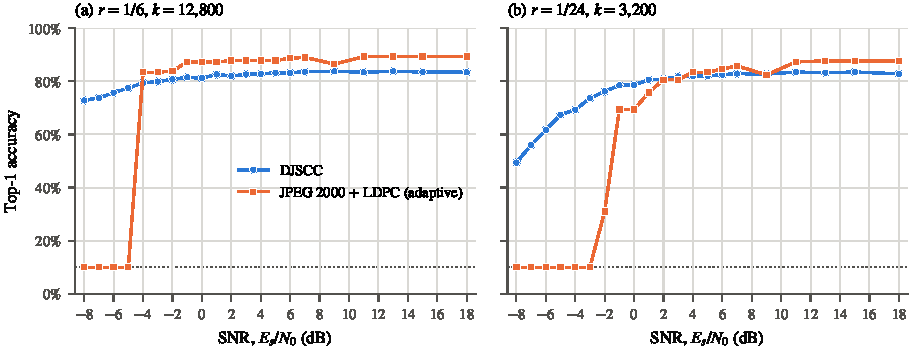
\includegraphics[width=\textwidth]{fig_bandwidth}
\caption{DJSCC against the adaptive JPEG~2000 baseline on the test split at two bandwidth ratios. (a) Three seed pairs with 95\% intervals; (b) the first seed pair. Reducing the channel uses fourfold moves the first SNR at which the digital system is ahead from $-2$~dB to $+2$~dB.}
\label{fig:s-bandwidth}
\end{figure*}

\begin{figure*}[t]
\centering
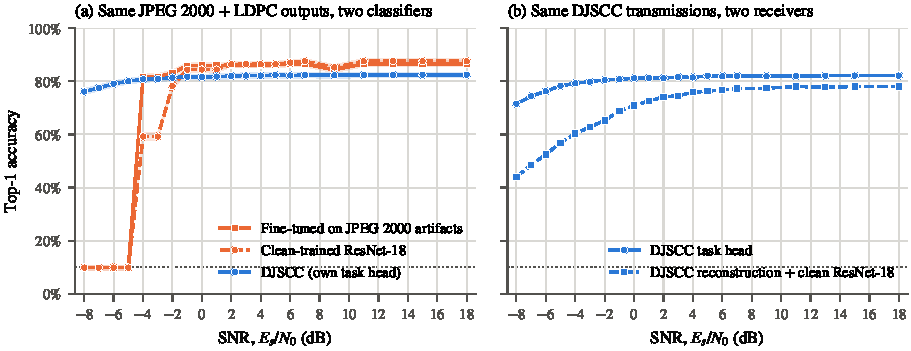
\includegraphics[width=\textwidth]{fig_scorer}
\caption{(a) The same JPEG~2000 + LDPC outputs at $r=1/6$ scored by the fine-tuned and the clean ResNet-18, with DJSCC for reference (three seed pairs). (b) The same DJSCC transmissions read by the DJSCC task head and by the clean ResNet-18 applied to the DJSCC reconstruction (first seed pair).}
\label{fig:s-scorer}
\end{figure*}

\begin{figure}[t]
\centering
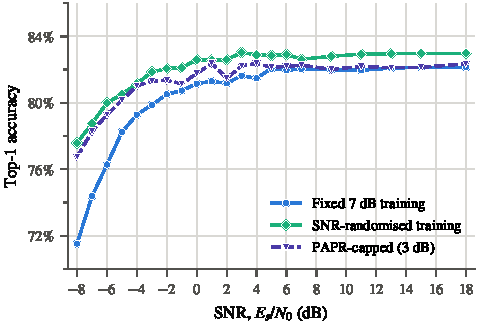
\includegraphics[width=\columnwidth]{fig_training}
\caption{DJSCC at $r=1/6$ on the test split, first seed pair: trained at a fixed 7~dB, trained with SNR drawn from $\{1,4,7,13,19\}$~dB, and trained with a 3~dB symbol PAPR cap. The other two seed pairs of the fixed-SNR model score 78.4\% and 78.5\% at $-8$~dB. Note the vertical scale.}
\label{fig:s-training}
\end{figure}

\begin{figure}[t]
\centering
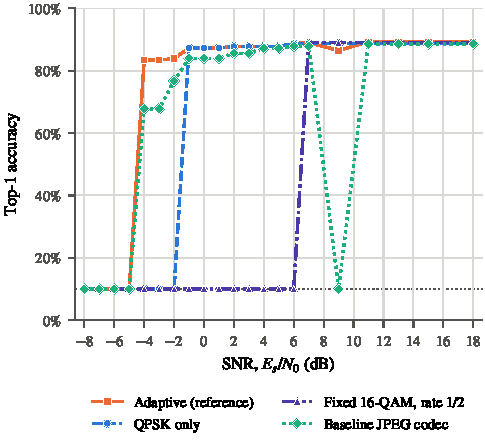
\includegraphics[width=\columnwidth]{fig_controls}
\caption{Adaptive JPEG~2000 + LDPC at $r=1/6$ on the test split against restricted versions: QPSK only (rate and resolution still adapted), one fixed operating point at all SNRs, and baseline JPEG in place of JPEG~2000. All scored by the fine-tuned ResNet-18.}
\label{fig:s-controls}
\end{figure}

\FloatBarrier
\section{Reproducing the Figures and Tables}
\label{sec:repro}

The figures and tables in the paper and in this document are regenerated from the committed result files, without model weights, datasets, or a GPU:

\begin{lstlisting}[language=bash,basicstyle=\ttfamily\scriptsize]
git clone https://github.com/nxck2005/capstone
cd capstone
python3 deliverables/research-paper/figures/make_figures.py
python3 deliverables/research-paper/supplement/make_tables.py
cd deliverables/research-paper
latexmk -pdf capstone_rp.tex
cd supplement && latexmk -pdf capstone_rp_supplement.tex
\end{lstlisting}

Both scripts read only committed files: \path{presentation-results/data/g12_test_*.csv}, \path{results/g12/}, and \path{results/learned/w10/w10_continuation_units_v11.json}. The two CSV tables are written by \path{tools/export_g12_tables.py} from the per-image test outcomes, which are archived outside the repository and bound by the digests in \path{results/per_image_manifest.csv}. Re-running training or evaluation requires the Imagenette-160 archive, an NVIDIA GPU, and the environment pinned in \path{requirements.lock}.

The test campaign itself ran once under the committed freeze manifest \path{results/freeze_manifest.json}. Its execution record is in \path{results/g12/}: \path{attempt1_abort_custody.json} documents a first launch that stopped before any model produced a test output, and \path{post_freeze_corrections/} records, with the exact files and contents changed, the two execution corrections described in Section~V-A of the paper. Neither changed a model, an operating point, a noise draw, an analysis rule, or a reported accuracy.

\section*{Acknowledgment}
This supplementary material was produced with Anthropic's Claude Opus~5.5. It wrote the pseudo-code in Section~S1 from the project's source code, selected and condensed the code excerpts in Section~S2, drafted the text throughout, and generated the tables in Sections~S3--S5 and the figures in Section~S6 with scripts that read the published result files. The code excerpted in Section~S2 was written with the assistance of Claude Opus~5.5 and OpenAI's GPT-5.6 Sol. All content was reviewed and verified by the authors, who take full responsibility for it.

\end{document}
